\chapter[Naissance des gènes impliqués dans une voie de signalisation humaine]{Article 1 - Naissance des gènes impliqués dans une voie de signalisation humaine}
\thispagestyle{firstpage}% Remplacez la valeur par celle recommandée par l'avertissement
\onehalfspacing

\section{Contexte de l'étude}
\par La communication cellulaire est un mécanisme important comme expliqué au Chapitre ~\ref{commcel}. Comme précédemment expliqué, une voie de signalisation s’initie principalement par la fixation d’un ligand sur son récepteur membranaire. C’est donc dans cette logique de poursuivre les travaux menés par Anna Grandchamp lors de son doctorat (2015-2018) qui portait sur le moment d’apparition des ligands et de leurs récepteurs membranaires dans l’arbre de la vie des métazoaires que cette étude a vu le jour. Nous nous sommes intéressés à l’ensemble des voies de signalisation intracellulaire, et nous avons étudié s’il existait un lien entre la position des protéines au sein d’une voie, et le moment d’apparition des gènes correspondants dans l’arbre de la vie. Cette étude est présentée sous forme de schéma récapitulatif en Figure ~\ref{fig:14_schéma1} page ~\pageref{fig:14_schéma1} et est suivie d’un article soumis page \pageref{art1}.

\section{Matériels et méthode}
\par Pour cette étude, comme pour la prochaine, nous avons récupéré un ensemble de 2 298 gènes uniques impliqués dans 47 voies de signalisation humaine dans la base de données KEGG V104. Les voies et leurs caractéristiques sont présentées dans le Tableau \ref{table:voiecaracteristiq}. 
\par Afin de déterminer le moment d’apparition, nous avons récupéré les arbres Genomicus Vertebrates V109 et Metazoa V51. Pour chacun de nos gènes, nous avons remonté l’arbre jusqu’à obtenir l’orthologue le plus ancien décrit. Le nœud le plus ancien regroupant l’espèce contenant l’orthologue de l’homme est alors noté comme étant le moment d’apparition du gène en question. Nous récupérons également toutes les interactions protéine-protéine pour regarder l’ordre d’apparition dans la voie, qu’il soit « \textit{backward} » (le membre impliqué en amont dans la voie (proche du couple ligand-récepteur) est arrivé en premier), « \textit{forward} » (le membre impliqué en aval dans la voie (proche d’un facteur de transcription) est arrivé en premier), ou simultanée (les deux membres sont apparus au même nœud évolutif). Et enfin, pour déterminer une éventuelle corrélation entre la position des protéines dans la voie et le moment de naissance du gène correspondant, nous avons récupéré l’ensemble des portions de voie que nous appelons “sous-voies“ d’une voie et attribué un rang à chaque gène en fonction de la position qu’il occupait dans cette sous-voie. Des tests de permutation ont été réalisés pour étudier si les relations \textit{forward}, \textit{backward} et simultanées étaient dues au hasard ou non, ainsi que des tests de corrélation (Pearson) pour vérifier que la relation position des gènes dans la voie (près de la membrane ou près de la cible, le plus souvent dans le noyau) et le nœud de naissance du gène dans l’arbre était liés. 

\section{Résultats}
\par Dans un premier temps, nous avons montré qu’il existait 2 principaux nœuds dans l’arbre de la vie à l’origine des gènes impliqués dans les voies de signalisation, à la racine des opisthocontes et à la racine des vertébrés. Concernant les interactions gène-gène, les partenaires ont des moments d’apparition le plus souvent asynchrone (83,87\%, dont 40,66\% de relation \textit{backward} et 43,21\% de relation \textit{forward}), contre 16,13\% de naissances simultanées pour les deux partenaires d’une interaction. Pour 12 voies, on retrouve une corrélation positive (p-value < 0,047) entre les positions dans la voie et les nœuds de naissance des gènes, ce qui voudrait dire que ces voies auraient une tendance à s’être construites du début de la voie (ligand-récepteur) vers l’aval de la voie (facteur de transcription). Donc pour 35 voies, il s'agirait de l'aléatoire qui primerait. 

\section{Conclusion}
\par Deux scénarios évolutifs semblent se dégager concernant la “construction“ des voies de signalisation humaine au cours de l’évolution et motivées par deux moments clés dans l’arbre de la vie des animaux : à la racine des Opisthocontes ainsi qu’à la racine des vertébrés. Pour 12 de nos voies de signalisation, elles se seraient plutôt construites de l’aval de la voie vers l’amont de la voie, et pour 35 autres, ce serait le scénario de l'aléatoire qui serait à l’origine de la construction de ces voies.

\begin{figure}[H]
    \centering
    \includegraphics[width=1\textwidth]{figures/corps/figure14.png}
    \caption{Schéma récapitulatif de l'étude 1}
    \label{fig:14_schéma1}
\end{figure}

\section{Article}\label{art1}
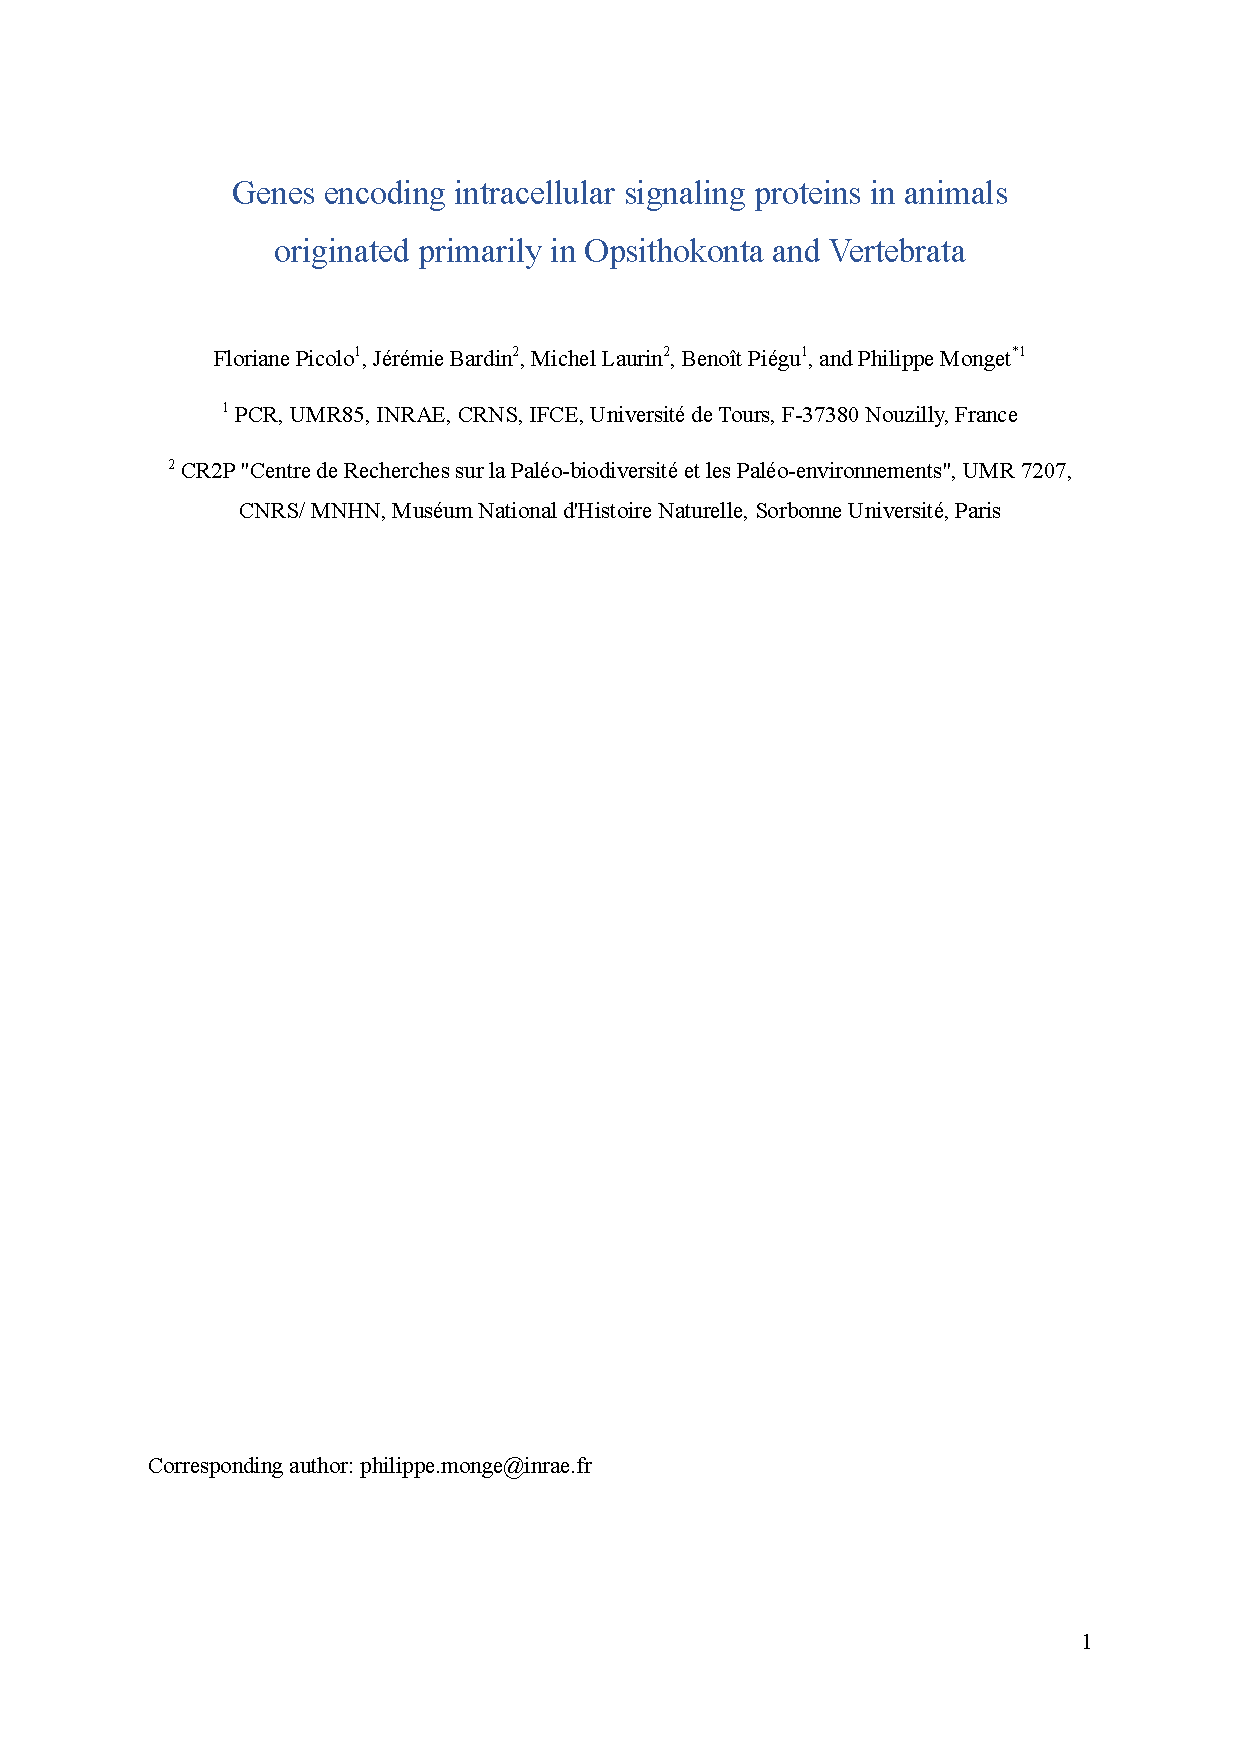
\includepdf[scale=0.9,pages=1-23,pagecommand={\thispagestyle{normalpage}}]{figures/articles/article1.pdf}

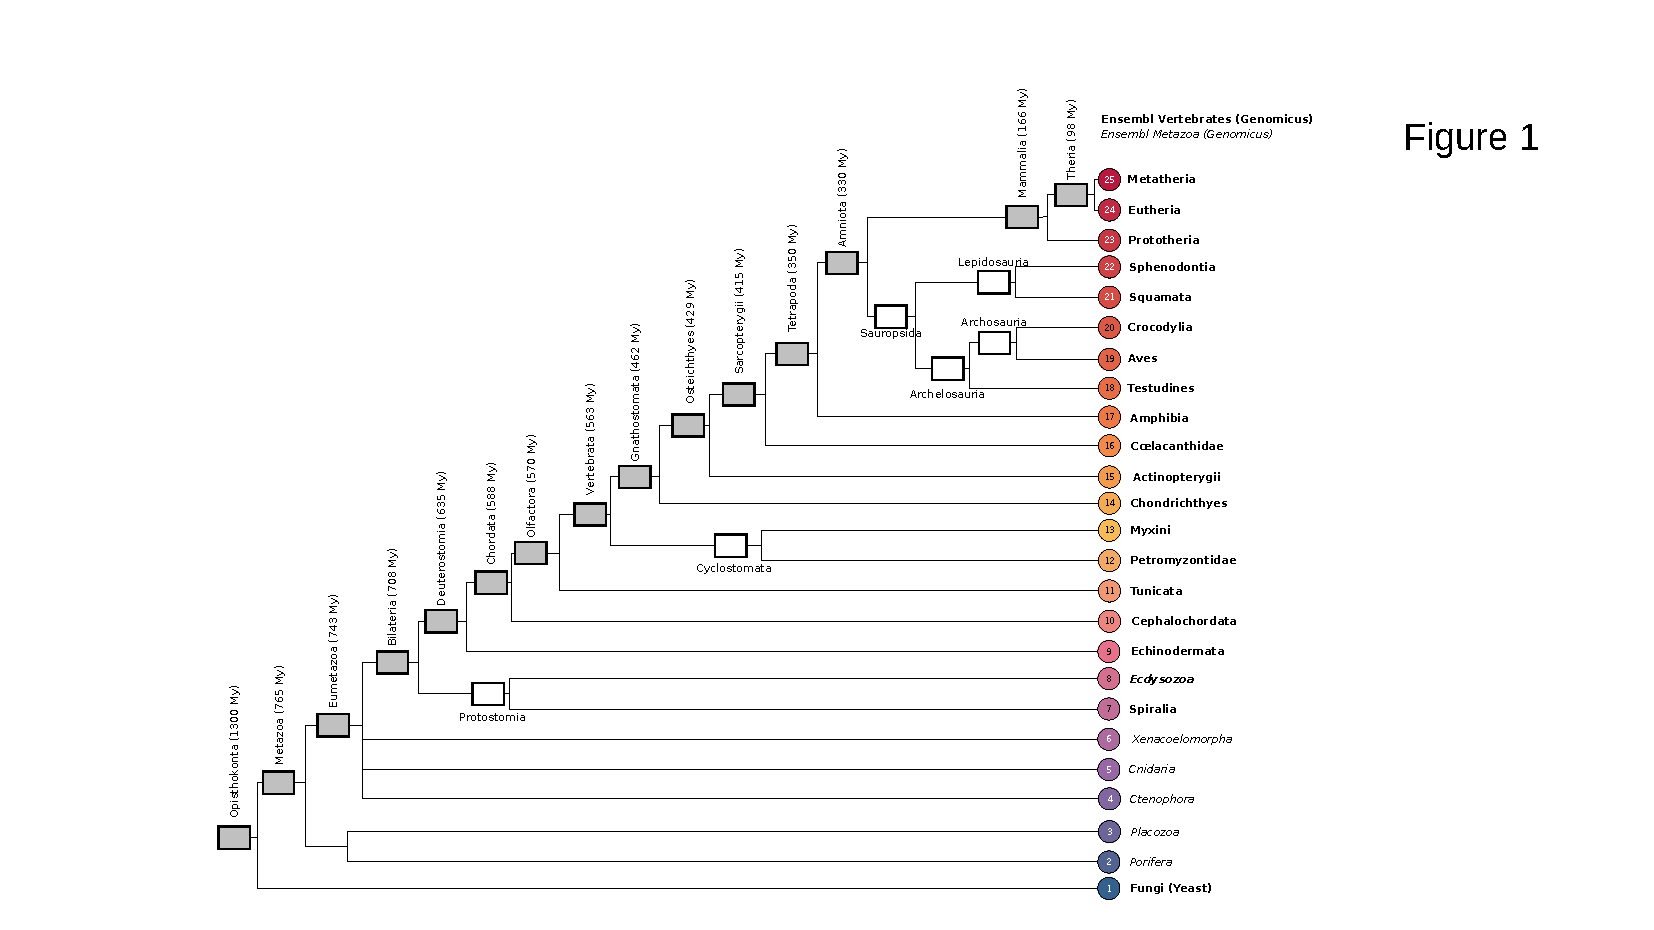
\includepdf[scale=0.80,pages=1-11, nup=1x2,pagecommand={\thispagestyle{normalpage}}]{figures/articles/figures-article1.pdf}
